\begin{figure}[t]
\centering
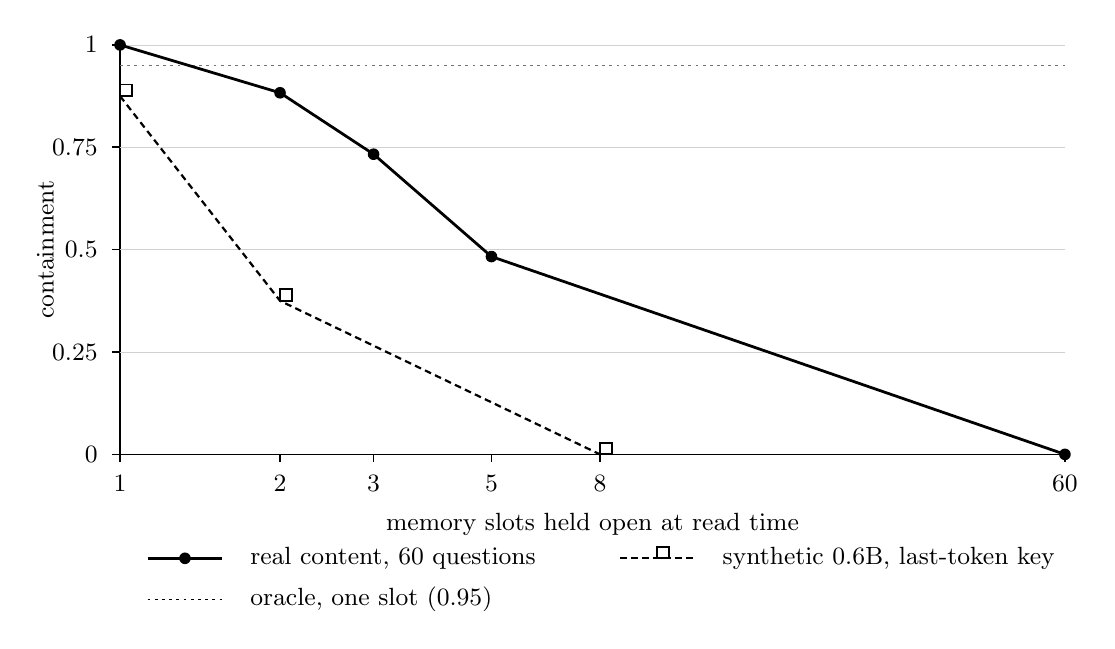
\begin{tikzpicture}[x=1cm,y=1cm]
  \draw[black,line width=0.6pt] (0,0) -- (12.00,0);
  \draw[black,line width=0.6pt] (0,0) -- (0,5.20);
  \draw[black!18,line width=0.3pt] (0,1.300) -- (12.00,1.300);
  \draw[black!18,line width=0.3pt] (0,2.600) -- (12.00,2.600);
  \draw[black!18,line width=0.3pt] (0,3.900) -- (12.00,3.900);
  \draw[black!18,line width=0.3pt] (0,5.200) -- (12.00,5.200);
  \draw[black,line width=0.6pt] (0.000,0) -- ++(0,-0.10);
  \node[below=0.14cm,font=\small] at (0.000,0) {1};
  \draw[black,line width=0.6pt] (2.032,0) -- ++(0,-0.10);
  \node[below=0.14cm,font=\small] at (2.032,0) {2};
  \draw[black,line width=0.6pt] (3.220,0) -- ++(0,-0.10);
  \node[below=0.14cm,font=\small] at (3.220,0) {3};
  \draw[black,line width=0.6pt] (4.717,0) -- ++(0,-0.10);
  \node[below=0.14cm,font=\small] at (4.717,0) {5};
  \draw[black,line width=0.6pt] (6.095,0) -- ++(0,-0.10);
  \node[below=0.14cm,font=\small] at (6.095,0) {8};
  \draw[black,line width=0.6pt] (12.000,0) -- ++(0,-0.10);
  \node[below=0.14cm,font=\small] at (12.000,0) {60};
  \draw[black,line width=0.6pt] (0,0.000) -- ++(-0.10,0);
  \node[left=0.16cm,font=\small] at (0,0.000) {0};
  \draw[black,line width=0.6pt] (0,1.300) -- ++(-0.10,0);
  \node[left=0.16cm,font=\small] at (0,1.300) {0.25};
  \draw[black,line width=0.6pt] (0,2.600) -- ++(-0.10,0);
  \node[left=0.16cm,font=\small] at (0,2.600) {0.5};
  \draw[black,line width=0.6pt] (0,3.900) -- ++(-0.10,0);
  \node[left=0.16cm,font=\small] at (0,3.900) {0.75};
  \draw[black,line width=0.6pt] (0,5.200) -- ++(-0.10,0);
  \node[left=0.16cm,font=\small] at (0,5.200) {1};
  \node[below=0.62cm,font=\small] at (6.00,0) {memory slots held open at read time};
  \node[rotate=90,above=0.72cm,font=\small] at (0,2.60) {containment};
  \draw[black!55,line width=0.5pt,dash pattern=on 1pt off 1.6pt] (0,4.940) -- (12.00,4.940);
  % synthetic, 0.6B, last-token key
    \draw[black,dash pattern=on 2.4pt off 1.6pt,line width=0.8pt] (0.000,4.550) -- (2.032,1.950) -- (6.095,0.000);
        \draw[black,line width=0.7pt,fill=white] (0.000,4.550) rectangle +(4.2pt,4.2pt);
        \draw[black,line width=0.7pt,fill=white] (2.032,1.950) rectangle +(4.2pt,4.2pt);
        \draw[black,line width=0.7pt,fill=white] (6.095,0.000) rectangle +(4.2pt,4.2pt);
  % real benchmark content, 60 questions
    \draw[black,line width=1.0pt] (0.000,5.200) -- (2.032,4.592) -- (3.220,3.812) -- (4.717,2.512) -- (12.000,0.000);
        \fill[black] (0.000,5.200) circle (2.1pt);
        \fill[black] (2.032,4.592) circle (2.1pt);
        \fill[black] (3.220,3.812) circle (2.1pt);
        \fill[black] (4.717,2.512) circle (2.1pt);
        \fill[black] (12.000,0.000) circle (2.1pt);
  % legend, outside the axes
  \draw[black,line width=1.0pt] (0.35,-1.32) -- (1.30,-1.32);
    \fill[black] (0.825,-1.320) circle (2.1pt);
  \node[right=0.16cm,font=\small] at (1.37,-1.32) {real content, 60 questions};
  \draw[black,dash pattern=on 2.4pt off 1.6pt,line width=0.8pt] (6.35,-1.32) -- (7.30,-1.32);
    \draw[black,line width=0.7pt,fill=white] (6.825,-1.320) rectangle +(4.2pt,4.2pt);
  \node[right=0.16cm,font=\small] at (7.37,-1.32) {synthetic 0.6B, last-token key};
  \draw[black,dash pattern=on 1pt off 1.6pt,line width=0.5pt] (0.35,-1.84) -- (1.30,-1.84);
  \node[right=0.16cm,font=\small] at (1.37,-1.84) {oracle, one slot (0.95)};
\end{tikzpicture}
\caption{Containment against the number of memory slots held open at read time, on a logarithmic axis. One slot is as good as the oracle; two already cost, and the loss grows monotonically until the whole bank is open, where $\tSum$ of the synthetic questions are answered. The real-content curve falls more gently than the synthetic one but never turns upward, so the generator exaggerates the size of the effect without creating it (Table~\ref{tab:t7collision}).}
\label{fig:collapse}
\end{figure}
